\begin{table}[h!]
\section{Anwendung der Differential- und Integralrechnung}

\begin{center}

% % % % % % % % % % % % % % % % % %
%Darstellungsformen
% % % % % % % % % % % % % % % % % %	
\begin{tabularx}{540pt}{|p{180pt}|p{180pt}|X|}
\hline
\rowcolor{Gray}
\multicolumn{3}{|c|}{\textbf{Darstellungsformen}}\\
\hline
Parameterform & Explizite Form & Implizite Form\\

$\begin{pmatrix}x(t)\\y(t)\end{pmatrix} = 
\begin{pmatrix}\Psi(t)\\\varphi(t)\end{pmatrix} $&
$y=f(x)$ \newline $r = f(\varphi)$&
$F(x,y) = 0$ \newline $F(\varphi, r) = 0$\\ 
\hline
\end{tabularx}	
		
% % % % % % % % % % % % % % % % % %
%Umrechnung verschiedener Systeme
% % % % % % % % % % % % % % % % % %	
\begin{tabularx}{540pt}{|p{150pt}p{120pt}X|}
	\hline
	\rowcolor{Gray}
	\multicolumn{3}{|c|}{\textbf{Umrechnung}}\\
	\hline

	Polar $\Leftrightarrow$ Kartesisch\newline
	(Falls Polgerade = x-Achse)&
	
	$x = r\cdot \cos\varphi$\newline
	$y = r\cdot \sin\varphi$&

	 $r^2 = x^2 + y^2$ \newline

 $\varphi =
  \begin{cases}\arctan(\frac{y}{x}) + \pi 	& x < 0\\
              \arctan(\frac{y}{x}) 	        & x > 0\\
              \frac{\pi}{2}			        & x = 0;\; y > 0\\
              -\frac{\pi}{2}		        & x = 0;\; y < 0\\
              \text{unbestimmt}		        & x = y = 0
  \end{cases}$\\
 \hline


\end{tabularx}

% % % % % % % % % % % % % % % % % %
% Kurvenarten
% % % % % % % % % % % % % % % % % %	
\begin{tabularx}{540pt}{|p{80pt}|p{180pt}|X|}
\hline
\rowcolor{Gray}
\multicolumn{3}{|c|}{\textbf{Kurvenarten}}\\
\hline


Polarform: &
`\textbf{+}`, Kurve auf linke Seite geöffnet&
`\textbf{-}` , Kurve auf rechte Seite geöffnet\\
\hline

&
\textbf{Kreis} & \textbf{Ellipse}\\

Implizit & 
$(x-x_0)^2 + (y - y_0)^2 = r^2$ &
$\left(\dfrac{x-x_0}{a}\right)^2 + \left(\dfrac{y-y_0}{b}\right)^2 = 1$\\

Polarform &
$r = \dfrac{p}{1 + \epsilon \cos(\varphi)}; \epsilon = 0$&
$r = \dfrac{p}{1 + \epsilon \cos(\varphi)}; 0 < \epsilon < 1 \qquad$ (rechter Brennpkt)\\

Parameterform&
$x=x_0 + R\cos(t), y=y_0 + R\sin(t) $ &
$x = a\cos(t); 
y = b\sin(t) \qquad$ um $P(0,0)$ \\

$p, \epsilon$&
$ p = \dfrac{b^2}{a}$&
$\epsilon = \dfrac{c}{a}$\\

\hline

&
\textbf{Hyperbel} & \textbf{Parabel}\\

Implizit & 
$\left(\dfrac{x}{a}\right)^2 - \left(\dfrac{y}{b}\right)^2 = 1$&
$y^2 = 2p(x-x_0)$\\

Polarform &
$r = \dfrac{p}{1 - \epsilon \cos(\varphi)}; \epsilon > 1_{(rechts)}$&
$r = \dfrac{p}{1 - \epsilon \cos(\varphi)}; \epsilon = 1$\\

Parameterform&
$x= a \cosh(t); y = b \sinh(t) $&
$x= \dfrac{t^2}{2p}; y = t$\\

&
&
$p=$Halbparameter (2$\cdot$Abstand Scheitel-Brennpunkt)\\
\hline

\multicolumn{2}{|c|}{
\textbf{Kardioide/Herzk.}:
$r = a(1+\cos(\varphi))$}&

\textbf{Lemniskate ``$\infty$'':}
$r = a\sqrt{2\cos(2\varphi)}$ \\
\hline
\multicolumn{2}{|c|}{
\textbf{Strophoide/harm. K.:}
$ r = -a \dfrac{\cos(2\varphi)}{\cos(\varphi)};(a>0) $ }&
\textbf{log. Spirale: }
$r=e^{a\varphi}$
\\
\hline
\end{tabularx}	

\end{center}
\end{table}	
	
	
\begin{table}[h!]
\begin{center}


% % % % % % % % % % % % % % % % % %
% Gleichungen
% % % % % % % % % % % % % % % % % %	
\begin{tabularx}{540pt}{|p{160pt}|p{180pt}|X|}
\hline
\rowcolor{Gray}
\multicolumn{3}{|c|}{\textbf{Gleichungen}}\\
	\hline
	linearer MW & absoluter MW (gleichrichtwert)  & quadratischer MW(Effektivwert) \\
	
	$\dfrac{1}{b-a}\int\limits_a^b f(x)dx$&
	$\dfrac{1}{b-a}\int\limits_a^b |f(x)|dx$&
	$\sqrt{\dfrac{1}{b-a} \int\limits_a^b |f(x)|^2 dx}$\\
	\hline

Tangentengleichung & Normalengleichung  & Hessesche Normalform \\

$y-y_0=m(x-x_0)$ &
$y-y_0=-\frac{1}{m}(x-x_0)$ &
$x\cdot \cos\varphi_0 +y\cdot \sin\varphi_0=r_0$ \\
\hline

Abstand zum Ursprung& Doppelpunkt& glatte Kurve(keine Ecken)\\

$\dfrac{|y_0 - m \cdot x_0|}{\sqrt{m^2 + 1}}$ &
$t_1 \neq t_2 \Rightarrow P(t_1)=P(t_2)$&
$\dot{\varphi(t)}^2+\dot{\psi(t)}^2\neq 0$\\
\hline

Länge Subtangente & Länge Subnormale& \\

$\dfrac{y_0}{|y_0'|}$&
$|y_0' \cdot y_0|$&
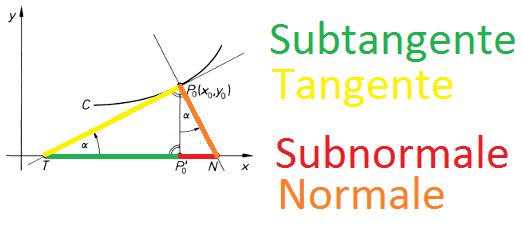
\includegraphics[width = 4cm]{bilder/3_tangent}\\
\hline

\multicolumn{3}{|c|}{
\parbox{450pt}{\textbf{Berührung in n-ter Ordnung:} Zwei explizit gegebene Kurven $y = f(x)$ und $y = g(x)$ berühren einander im
Punkt P $x_0, y_0$ von der Ordnung $n$, wenn die Funktionswerte und die ersten
$n$ Ableitungen existieren und übereinstimmen.\\
$f(x_0) = g(x_0);\; f'(x_0) = g'(x_0);\; f''(x_0) = g''(x_0);\;\ldots ;
\;f^{(n)}(x_0) = g^{(n)}(x_0)\; \qquad f^{(n+1)}(x_0) \neq g^{(n+1)}(x_0)$\\
Für annäherung von Polynom an beliebige Kurve}}\\
\hline
\end{tabularx}

% % % % % % % % % % % % % % % % % %
% Kartesisch - Parameter - Polar
% % % % % % % % % % % % % % % % % %	
\begin{tabularx}{540pt}{|p{120pt}|p{170pt}|X|}
\hline
\rowcolor{Gray}
\textbf{Kartesisch} & \textbf{Parameter} & \textbf{Polar}\\
\hline
		\multicolumn{3}{| l |}{\textbf{Anstieg einer Kurve, Ableitung, 2. Ableitung}} \\
    	\hline   
    	$y'=f'(x_o) \quad y'' = f''(x_0)$ & 
    	$y'=\dfrac{\dot{y}}{\dot{x}} \quad 
    	y'' = \dfrac{\dot{x} \ddot{y} - \dot{y}\ddot{x}}{\dot{x}^3}$ &
    	$y'=\dfrac{r'(\varphi) \sin(\varphi) + r(\varphi) \cdot
    	\cos(\varphi)}{r'(\varphi) \cos(\varphi)-r(\varphi) \cdot \sin(\varphi)}$
    	\\
		
		\hline
		\multicolumn{3}{| l |}{\textbf{Bogenlänge }} \\
    	\hline
    	$s=\int\limits_a^b{\sqrt{1+(f'(x))^2}dx}$ & 
    	$|s|=\int\limits_{t_1}^{t_2}{\sqrt{\dot{x}^2(t)+\dot{y}^2(t)}dt}$ &
		$|s|=\int\limits_{\varphi_1}^{\varphi_2}{\sqrt{(r'(\varphi))^2+(r(\varphi))^2}d\varphi}$\\
		
		\hline		
		\multicolumn{3}{| l |}{\textbf{Krümmung ebener Kurven }  
		$\qquad$ $\frac{\Delta\alpha}{\Delta s}$
		$\qquad$ Scheitel bei: $K'(x)=0 \qquad$ und $\qquad K''(x)\neq 0
		\begin{cases}
		K(x)<0 & \text{Maxima}\\
		K(x)>0 & \text{Minima}
		\end{cases}$}\\
    	\hline
    	$\kappa=\dfrac{f''(x)}{(\sqrt{1+(f'(x))^2})^3}$ &
    	$\kappa=\dfrac{\dot{x}(t)\ddot{y}(t)-\dot{y}(t)\ddot{x}(t)}{(\sqrt{(\dot{x}(t))^2+(\dot{y}(t))^2})^3}$ &
		$\kappa=\dfrac{2(r'(\varphi))^2-r(\varphi)r''(\varphi)+(r(\varphi))^2}{(\sqrt{(r'(\varphi))^2+(r(\varphi))^2})^3}$\\   	
		
		\hline
		\multicolumn{3}{| l |}{Konvex (Linkskurve): $\kappa \geq 0 \qquad$ Streng
		konvex: $\kappa > 0 \qquad$ Wendepunkt: $\kappa = 0 \qquad$ Analog für konkav}\\
		
		\hline
		\multicolumn{3}{| l |}{\textbf{Krümmungskreisradius } $\qquad r = |\frac{1}{\kappa}|$} \\
		\hline
		$r = \left|\dfrac{(\sqrt{1+(f'(x))^2})^3}{f''(x)} \right|$ &
		$r = \left|\dfrac{(\sqrt{(\dot{x}(t))^2+(\dot{y}(t))^2})^3}
		{\dot{x}(t)\ddot{y}(t)-\dot{y}(t)\ddot{x}(t)} \right|$ & 
		$r = \left|\dfrac{(\sqrt{(r'(\varphi))^2+(r(\varphi))^2})^3}
		{2(r'(\varphi))^2-r(\varphi)r''(\varphi)+(r(\varphi))^2} \right|$ \\
\hline
\end{tabularx}


\end{center}
\end{table}	

% % % % % % % % % % % % % % % % % %
% neue Seite
% % % % % % % % % % % % % % % % % %	


\begin{table}[h!]
\begin{center}


\begin{tabularx}{560pt}{|p{170pt}|p{140pt}|X|}


\hline
\rowcolor{Gray}
\textbf{Kartesisch} &\textbf{Parameter} & \textbf{Polar}\\

		
		\hline		
		\multicolumn{3}{| l |}{\textbf{Flächeninhalt } um x-Achse $\qquad$y-Achse: Umkerhfunktion $f^{-1}(x)$ von $y_0$ bis $y_1$ integrieren} \\
    	\hline
    	$A=\int\limits_a^b{f(x)}dx$  & 
    	$A=\frac{1}{2}\int\limits_{t_1}^{t_2}{[x\dot{y}-\dot{x}y]dt}$ &
		$A=\frac{1}{2}\int\limits_{\varphi_1}^{\varphi_2}{r^2d\varphi}$\\  
    	
		\hline		
		\multicolumn{3}{| l |}{\textbf{Volumen } $\qquad$ \textbf{Symmetrie!} nur 1.Hälfte der Kurve integrieren (pos. Meridian)} \\
    	\hline
		$V=\pi\int\limits_a^b(f(x))^2dx$ & 
    	$V=\pi\left|\int\limits_{t_1}^{t_2}{y^2\dot{x}dt}\right|$ &
		$V=\pi\left|\int\limits_{\varphi_1}^{\varphi_2}{r^2\sin^2\varphi[r'\cos(\varphi)-r\sin(\varphi)]d\varphi}\right|$\\  
    	
		\hline		
		\multicolumn{3}{| l |}{\textbf{Oberflächeninhalt } $\qquad$ \textbf{Symmertire!} nur 1.Hälfte der Kurve integrieren (pos. Meridian)} \\
    	\hline
   		$O=2\pi\int\limits_a^b{|f(x)|\sqrt{1+(f'(x))^2}dx}$ & 
    	$O=2\pi\int\limits_{t_1}^{t_2}{|y|\sqrt{\dot{x}^2+\dot{y}^2}dt}$ &
		$O=2\pi\int\limits_{\varphi_1}^{\varphi_2}{|r\sin\varphi|\sqrt{(r')^2+r^2}d\varphi}$\\  
    	\hline
		\multicolumn{3}{| l |}{Polar: \qquad $\sin \varphi =$ Drehung um Polgerade \qquad $\cos y =$ Drehung um y-Achse $(f = \frac{\pi}{2}) \qquad \rightarrow$ siehe Fläche} \\
	\hline
		\multicolumn{3}{| l |}{\textbf{Krümmungskreismittelpunkt}} \\
	\hline
		$x_c = x - \dfrac{\frac{dy}{dx}[1 + (\frac{dy}{dx})^2]}{\frac{d^2y}{dx^2}}$&
		$ x_c = x - \dfrac{\dot{y}(\dot{x}^2 + \dot{y}^2)}{\dot{x}\ddot{y} - \ddot{x}\dot{y}} $ &
		$x_c = r\cdot \cos\varphi - \dfrac{(r^2 + r'^2)(r\cdot \cos\varphi + r' \cdot \sin\varphi)}{r^2 + 2r'^2 - r\cdot r''}$\\

		$y_c = y + \dfrac{1+ (\frac{dy}{dx})^2}{\frac{d^2y}{dx^2}}$&
		$y_c = y + \dfrac{\dot{x}(\dot{x}^2 + \dot{y}^2)}{\dot{x}\ddot{y} - \ddot{x}\dot{y}} $ &
		$y_c = r\cdot \sin\varphi - \dfrac{(r^2 + r'^2)(r\cdot \sin\varphi - r' \cdot \cos\varphi)}{r^2 + 2r'^2 - r\cdot r''}$\\
		\hline
		\multicolumn{3}{|l|}{Umrechnung Kart $\Leftrightarrow$ Komp.:
		 $x(t)$ , $ y(t)$ und $ \int f(x)dx \Rightarrow \qquad dx=\dot{x}dt \Rightarrow \qquad \int y(t)\dot{x}(t)dt$}\\
	\hline

\end{tabularx}


\end{center}
\end{table}	
	